Pro potřeby této práce byly vytvořeny 2 aplikace a 2 knihovny. První aplikace je
demonstrační aplikací k~měřicímu vozu, tato aplikace pouze zobrazuje naměřená
data. Druhá aplikace je o~mnoho komplexnější a řeší přímo problém automatické
kalibrace.

\section{Volba nástrojů}
\label{sec:sw-nastroje}

Zásadní otázkou, kterou je třeba zodpovědět před vytváření programu, je
jaký programovací jazyk a případně framework zvolit. Zde měl autor poměrně
jasný požadavek na programovací jazyk: jazyk musí mít poměrně silný typový
systém tak, aby netriviální množství kontrol proběhlo již během překladu.
Důvodem pro tento argument je fakt, že autor vyrábí aplikaci, které je tzv.
\textit{kritická}. V~kontextu této práce to znamená, že vlivem chyby
v~aplikaci může dojít k~materiálním škodám na kalibrovaném modelu (ceny
vybraných malosériových modelů se pohybují až v~desítkách tisíc Kč).

Dalším přirozeným požadavkem bylo, aby programovací jazyk měl rozumnou podporu
pro komunikaci se sériovým portem, neboť toto rozhraní bude použito jak pro
komunikaci s~měřicím vozem, tak pro komunikaci s~digitální centrálou DCC.

Dalším kritériem při výběru programovacího jazyka byla jeho předchozí znalost
autorem práce. Zejména u~kritických aplikací je totiž nanejvýš důležité, aby
programátor přesně věděl, co dělá.

Při rozmýšlení nad technologií aplikace bylo rozhodnuto, že program by měl
mít grafické uživatelské rozhraní (GUI), neboť je nanejvýš vhodné zobrazovat
přehledně aktuální průběh kalibrace a neboť jsou běžní uživatelé na GUI
aplikace zvyklí.

Zásadní je pak otázka typu aplikace. Autor uvažoval aplikace desktopové,
mobilní, webové a dokonce i~embedded! Embedded aplikace s~sebou nesou tu
nevýhodu, že obsluha s~aplikací typicky nemůže příliš interagovat, u~mobilních
aplikací je v~kontextu této práce omezující zejména zobrazovací plocha
zařízení, na kterou se jednoduše nevejde tolik dat, kolik by aplikace chtěla
zobrazovat. Navíc vývoj pro jiné zařízení, než na kterém se kód píše, vždy
přináší nějakou režii navíc.

Výhodou webové aplikace by byla snadná přenositelnost na jiné počítače,
aplikace by dokonce mohla být přístupná i~z~mobilního zařízení. Bohužel, proti
tomuto formátu aplikace hovoří fakt, že autor práce nemá s~webovými aplikacemi
dostatečné zkušenosti a už vůbec si netroufá v~nich psát kritický kód.
Oproti desktopovým aplikacím jsou interaktivní webové aplikace navíc o~něco
složitější (zejména co se týče předávání signálů z~GUI).

Další možností pak byly desktopové aplikace. Vzhledem k~požadavkům uvedeným
výše a k~faktu, že se jedná už o~poněkud rozsáhlejší projekt, jako nejvhodnější
se autorovi jevil jazyk \texttt{C++} s~použitím frameworku \texttt{Qt}.
Argumentem pro tento framework byly dobré osobní reference, které na
\texttt{Qt} autor práce dostal od kolegů. Ukázalo se také, že \texttt{Qt} poskytují
nejen výbornou multiplatformní podporu pro GUI, ale také stejně dobrou
multiplatformní podporu pro sériový port. Bylo tedy rozhodnuto, že výsledná
aplikace bude psána v~programovacím jazyce \texttt{C++} (konkrétně
\texttt{C++14}) za použití frameworku \texttt{Qt} a bude multiplatformní
(minimálně mezi OS \texttt{Windows} a \texttt{Linux}).

\section{WSM Speed Reader}
\label{sec:sw-wsm-speed-reader}

První aplikací je \textit{WSM Speed Reader} -- jednoduchý zobrazovač vyčtených
dat. Aplikace se skládá z~jednoho okna a je především typu
\textit{proof of concept}. GUI aplikace je zachyceno na obrázku
\ref{fig:wsm-speed-reader-gui}.

\begin{figure}[h]
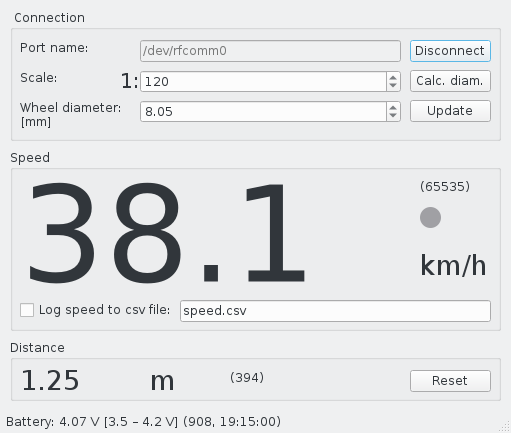
\includegraphics[width=0.7\textwidth]{data/speed_reader_screenshot.png}
\caption{GUI programu WSM Speed Reader.}
\label{fig:wsm-speed-reader-gui}
\end{figure}

Aplikace se připojuje k~sériovému portu, ze zadaných parametrů vypočítává
rychlost a ujetou vzdálenost vozidla a tyto údaje zobrazuje. Umožňuje ukládání
vyčtených dat do souboru (především pro vývoj) a ukládání nastavení aplikace
do konfiguračního souboru. Aplikace je volně dostupná pod licencí Apache
License v2.0 \cite{wsm-speed-reader}.

Při programování této aplikace bylo rozhodnuto vyčlenit knihovnu umožňující
komunikaci s~měřicím vozem WSM do samostatného repozitáře. Knihovna se skládá
hlavičkového souboru \texttt{wsm.h}, který definuje API třídy \texttt{Wsm},
implementace této knihovny (v~samostatném \texttt{cpp} souboru) a pomocných
souborů. Knihovna je k dispozici
online\footnote{\url{https://github.com/kmzbrnoI/wsm-lib-cpp-qt}}, bylo k ní
vytvořeno srozumitelné README a dodány všechny náležitosti samostatné stojícího
projektu.

I přes původní snahy je nutné pro užití knihovny v projektu využít frameworku
\texttt{Qt} a to zejména kvůli implementaci sériového portu.

\section{Automatic Calibration}
\label{sec:sw-wsm-auto-calib}

Program \textit{Automatic Calibration} umožňuje automaticky provést proces
kalibrace. V souladu s požadavky kladenými na výsledné sofwarové řešení
umožňuje

\begin{compactitem}
\item připojení k centrále XpressNET a měřicímu vozu WSM,
\item ruční řízení libovolnho hnacího vozidla,
\item vyčítání základních CV lokomotivy,
\item načtení závislosti rychlostní stupeň -- rychlost ze souboru dle požadavků
uživatele,
\item plně automatickou kalibrace rychlostní tabulky,
\item poloautomatickou kalibraci brzdných křivek,
\item konfiguraci parametrů kalibrace konfiguračním suborem,
\item zobrazení průběhu kalibrace a umožnění přerušení a obnovení kalibrace,
\item načtení a uložení profilu lokomotivy do souboru,
\item zobrazení grafu závislosti rychlosti na výkonu motoru.
\end{compactitem}

Grafické uživatelské rozhraní aplikace je zachyceno na obrázku \ref{fig:ac-gui}.

\begin{figure}[h]
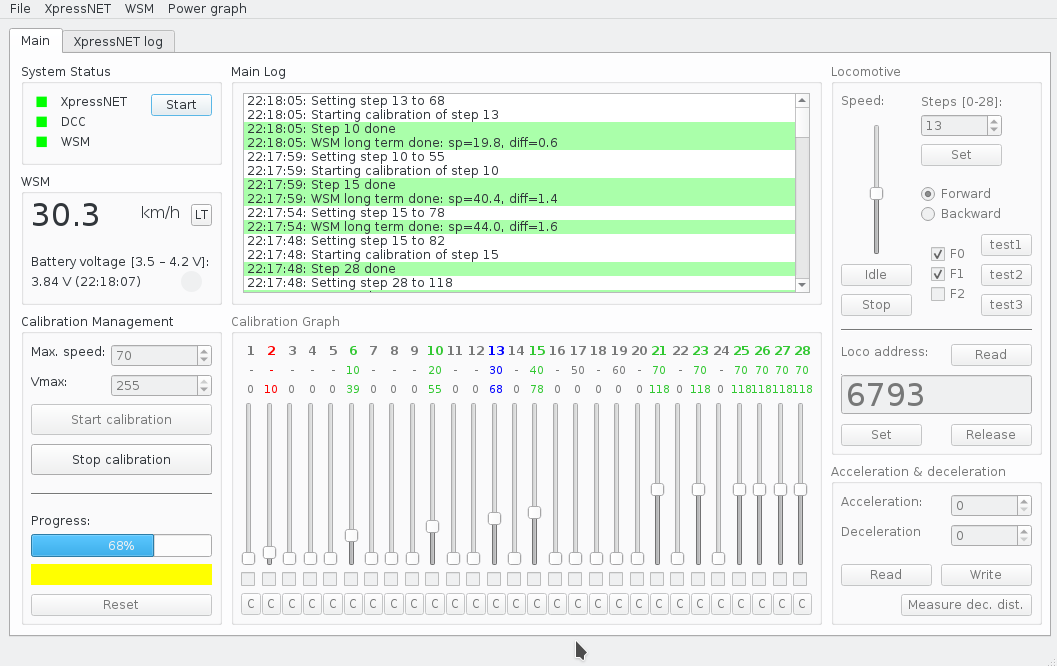
\includegraphics[width=\textwidth]{data/ac_progress.png}
\caption{Hlavní okno programu Automatic Calibration.}
\label{fig:ac-gui}
\end{figure}

Veškeré programování probíhá v režimu \textit{POM} (\textit{Programming on
Main}), který umožňuje, ačkoliv se nepředpokládá, že se tato možnost využije,
programování za plného provozu kolejiště.\footnote{DCC centrála umí programovat
dekodér ve dvou režimech: (1) programování na programovací koleji, (2)
\textit{Programming on Main -- POM}. Jedině na programovací koleji lze vyčítat
CV, při zvolení režimu \textit{POM} není možné přenášet data z lokomotivy zpět
do centrály.  Lokomotiva tedy ani nepotvrdí přijetí dat, centrála ale předem
počítá s případnou nespolehlivostí sbírání a proto radši posílá POM příkazy
dekodéru několikrát.  V praxi se problém chybějící odezvy neukazuje zásadní.
Při programování na prog.  koleji také typicky není možný provoz na kolejišti.}
Režim \textit{POM} byl zvolen zejména z toho důvodu, že při programování není
lokomotivu nutné zastavovat (oproti programování na prog. koleji), takže
kalibrace rychlostí může být výrazně rychlejší.

Aplikace je postavená na objektovém modelu, v aplikaci je několik tříd
založených na modelu \textit{singleto}, kde každá třída má jednu konkrétní
odpovědnost. Diagram tříd je zobrazen na obrázku
\ref{ac-classes}.

\begin{figure}[h]
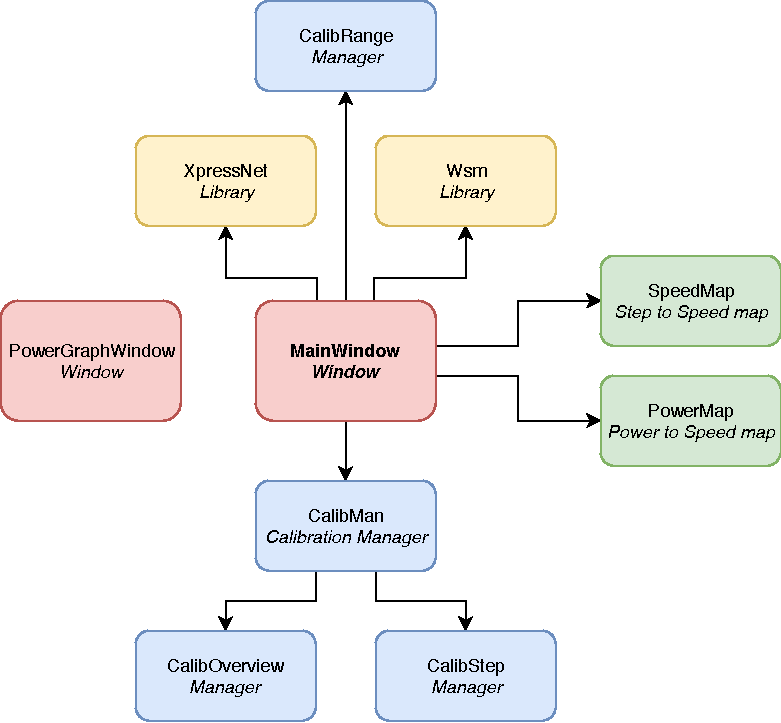
\includegraphics[width=0.7\textwidth]{data/ac_classes.pdf}
\caption{GUI programu WSM Speed Reader.}
\label{fig:ac-classes}
\end{figure}

Centrální třídou je třída obsluhující hlavní okno (\texttt{MainWindow}),
v~projektu jsou dále knihovny umožňující komunikaci s periferiemi (žluté),
nad těmito knihovnami jsou správci kalibrace (modré třídy). V projektu jsou
dále pomocné třídy (zelené), které jsou využívány v prakticky celé aplikaci.
Projekt je navržen tak, aby pouze červené třídy byly propojené s GUI, zbylé
třídy mezi sebou komunikují pomocí volání funkci a Qt signálů.

Třída \texttt{SpeedMap} udržuje mapu \textit{rychlostní stupeň: žádaná rychlost},
třída \texttt{PowerMap} pak udržuje mapu \textit{výkon motoru: reálná rychlost}.

O kalibraci rychlostních křivek se stará třída \texttt{CalibMan}. Kalibrace
je rozdělena do několika fází.

\begin{compactenum}
\item Zapsání základních CV.
\item Program si vytvoří základní přehled o tvaru křivky \textit{výkon motoru:
      reálná rychlost}.
\item Kalibrace jednotlivých jízdních stupňů.
\item Interpolace nekalibrovaných stupňů.
\end{compactenum}

Před začátkem kalibrace je nutné mít v SW načtenou mapu \textit{rychlostní
stupeň: žádaná rychlost}. Tato mapa je načítána z \texttt{csv} souboru a je
možné definovat v ní pouze nějaké jízdní stupně. Zbylé jízdní stupně se
interpolují ze sousedních nakalibrovaných hodnot nebo se nastaví manuálně.
Tato mapa je vlastností kolejiště, proto se načítá jen jednou.

Před kalibrací navíc uživatel zadá maximální kalibrovanou rychlost. Tato rychlost
je vlastností konkrétního hnacího vozidla, proto je možné ji ovlivnit před
každou jednotlivou kalibrací. Maximální rychlost spolu s akcelerací a decelerací
a oběma mapami jsou ukládány do \texttt{xml} souboru definice hnacího vozidla,
jehož formát byl záměrně převzat ze SW JMRI \ref{CITE}, aby bylo možné soubory
mezi těmito programy navzájem přenášet.

Další parametry, jako je například umístění zařízení sériového portu centrály
či maximální povolená odchylka kalibrace jsou načítání z jediného společného
konfiguračního souboru.

\subsection{Měření rychlosti}
\label{sec:ac:lt-measure}

Měření rychlosti během kalibrace probíhá ve speciálním režimu \textit{LT --
Long Term Measure}. Tento speciální režim je vlastností knihovny pro komunikaci
s měřicím vozem a umožňuje průměrování naměřených rychlostí. Bystrý čtenář si
jistě všimne, že autor právě představuje druhou vrstvu průměrování dat z
měřicího vozu (první probíhá již přímo ve vozu). Ano, je to tak. Ovšem cílem
průměrování na úrovní SW není pouze eliminovat oscilace rychlosti, výstupem
průměrování je totiž kromě průměrné rychlosti také rozdíl $v_{max} - v_{min}$ v
měřeném intervalu. Tento jakýsi \uv{pseudorozptyl} umožňuje kalibračnímu SW
považovat měření za relevantní pouze v případě, že rozptyl je dostatečně malý.
A přesně to kalibrační SW dělá.

Průměrování typicky probíhá pro $30$ naměřených rychlostí, tedy po dobu $3\ s$.

Kdykoliv je rozdíl $v_{max} - v_{min}$ naměřených rychlostí příliš velký
(konstanta je konfigurovatelná v nastavení, výchozí nastavení je $3\ km/h$, je
měření ignorováno a inicializováno měření nové. Pokud se takto několikrát
nepovede změřit rychlost (opět konfigurovatelná konstanta), je proces kalibrace
přerušen. Tento jen může být způsoben například nekvalitním vozidlem (a takové
vozidlo prostě odmítneme zkalibrovat) nebo například členitostí trati --
přítomností oblouků, stoupání a klesání, s kterými se BEMF nevyrovná.

\subsection{Fáze kalibrace rychlosti}

\subsubsection{Zapsání základních CV}

V této krátké fázi program nastaví do lokomotivy základní CV. Vypne rozjezdy a
dojezdy a nastaví škálovací parametry rychlostních křivek\footnote{Některé
dekodéry umožňují navíc zadat parametr, který určuje, jaké reálné střídě
signálu udpovídá hodnota $255$ výkonu motoru, čímž chtějí umožnit
škálování celé rychlostní tabulky bez nutnosti změnit výkon odpovídající
každému rychlostnímu stupni.} tak, aby výkony $0$--$255$ reálně pokrývaly celé
spektrum stříd signálů do motoru.

\subsubsection{Vytvoření přehledu}

O tento krok se stará třída \texttt{CalibOverview}.
Lokomotivě je nastaven rychlostní stupeň $2$ a na tento stupeň je zapsán výkon
$10/255$. Následně proběhne měření rychlosti. Dokud je rychlost lokomotivy
příliš malá, výkon je postupně zdvojnásobován a do mapy \textit{výkon:
rychlost} jsou přidávány nové záznamy. Jakmile se lokomotiva rozjede na
rychlost $> v_{min}$, program má informaci o tom, který rychlostní stupeň
odpovídá minimální rychlosti lokomotivy a přechází do další fáze.

V další fázi zkouší program výkony řádově $64-255$ a dokud nenaměří rychlost
vyšší než je uživatelem zadaná maximální rychlost, zkouší dál.

Na konci této fáze má program představu o tom, kterému rychlostnímu stupni
odpovídá minimální rychlost a kterému maximální rychlost.

V této fázi je rychlost lokomotivy měřena v režimu \textit{LT} (viz kapitolu
\ref{sec:ac:lt-measure}).

\subsubsection{Kalibrace jízdních stupňů}

Třída \texttt{CalibStep} umožňuje zkalibrovat jeden jízdní krok. Třída
\texttt{CalibMan} pak postupně volá třídu \texttt{CalibStep} dokud nejsou
zkalibrovány všechny jízdní kroky, které si uživatel přál zkalibrovat.

Kalibrace jednoho kroku probíhá následovně.

\begin{compactenum}
\item V mapě \textit{výkon: rychlost} je vyhledán (interpolován) výkon odpovídající
      kýžené rychlosti.
\item Výkon je zapsán do lokomotivy k právě kalibrovanému stupni.
\item Čekání $2\ s$ na změnu rychlosti lokomotivy.
\item Inicializace měření \textit{LT}.
\item Naměřenou hodnotu přidat do mapy \textit{výkon: rychlost}.
\item Pokud je rychlost v $\epsilon$ toleranci (konstantní konfigurovatelná hodnota)
      cílové rychlosti, krok je zkalibrován, jinak \texttt{GOTO krok 1}.
\end{compactenum}

$\epsilon$ je ve výchozím nastavení $1\ km/h$.

Jakmile je zkalibrována rychlost, kterou chceme na více rychlostních stupních,
jsou i tyto rychlostní stupně nastaveny na právě zkalibrovaný výkon.

Průběh kalibrace je průběžně zobrazován uživateli, uživatel vidí, které rychlostní
stupně jsou již zkalibrovány a které ještě ne.

\subsubsection{Interpolace}

Po dokončení kalibrace všech bodů zadaných v mapě \textit{rychlostní stupeň:
rychlost} jsou zbylé body postupně interpolovány.

Po dokončení této fáze zůstává typicky nezkalibrována minimální rychlost
(měřicí vůz neumí dobře měřit hodně malé rychlosti), pro kterou v \textit{Klubu
modelářů železnic Brno I} platí úzus, že je to taková nejnižší rychlost, při
které se hnací vozidlo již začne plynule pohybovat.  Po dokončení kalibrace
tedy uživatel ručně vybere rychlostní stupeň $1$ a nastaví jej na požadovanou
hodnotu za současného pozorování pohybu vozidla.

Program se pak postará o to, aby byly stupně do nejbližšího již zkalibrovaného
stupně interpolovány.
